\documentclass{standalone}
\usepackage{tikz}
\usetikzlibrary{patterns, positioning}

\begin{document}
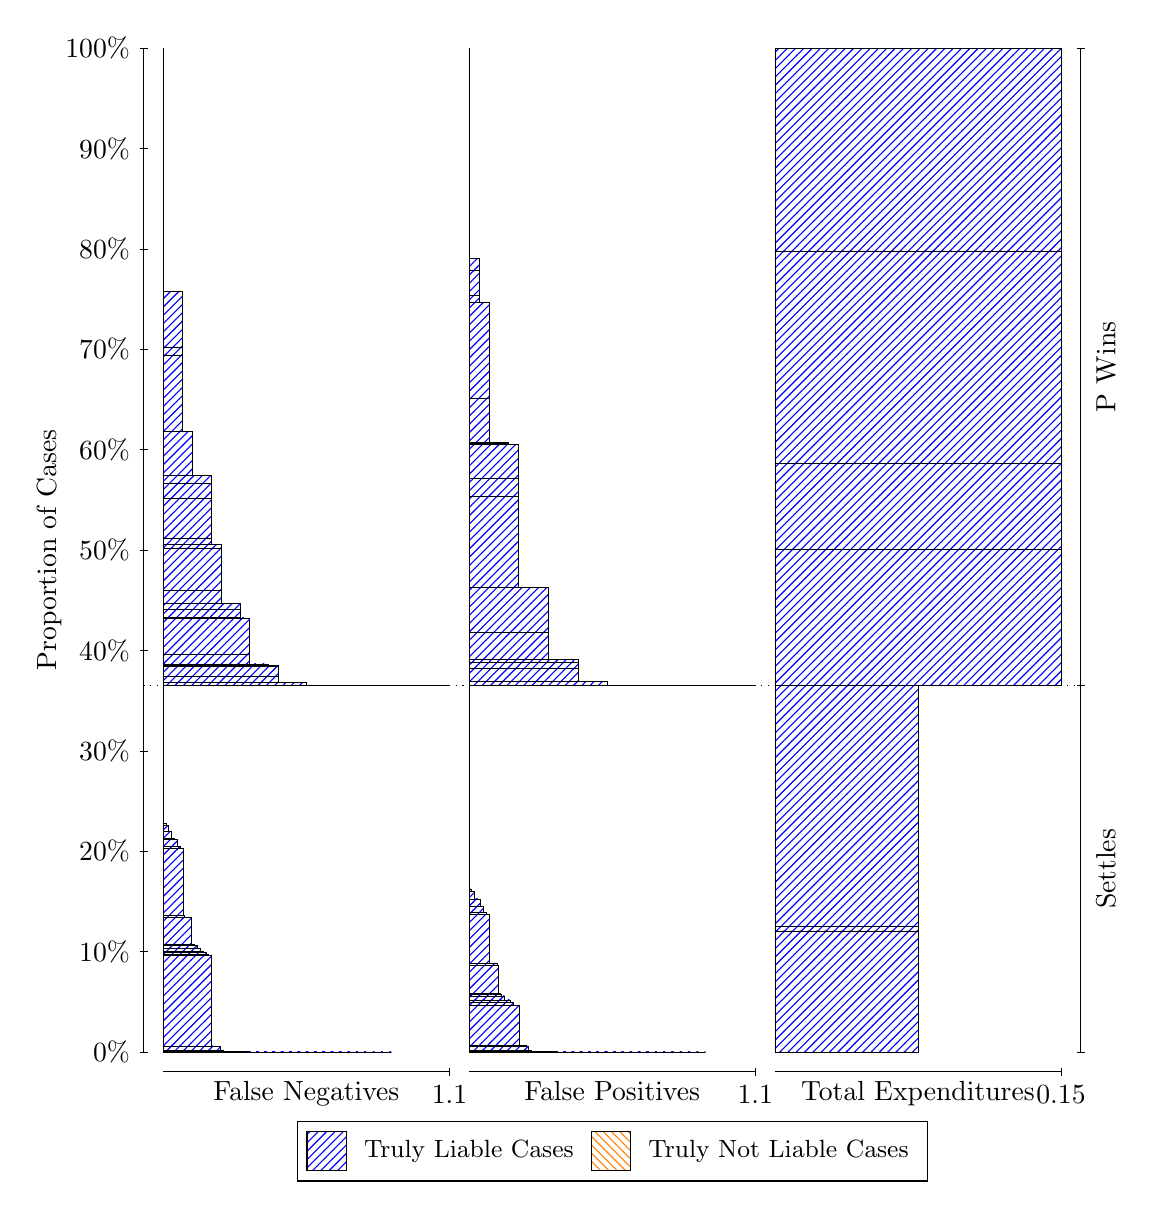
\begin{tikzpicture}
\draw[black, very thin] (1.5,1.75) -- (1.5,14.5);
\node[rotate=90, anchor=center] at (0.3, 8.125) {Proportion of Cases};
\draw[black, very thin] (1.45,1.75) -- (1.55,1.75);
\node[anchor=east] at (1.45, 1.75) {0\%};
\draw[black, very thin] (1.45,3.025) -- (1.55,3.025);
\node[anchor=east] at (1.45, 3.025) {10\%};
\draw[black, very thin] (1.45,4.3) -- (1.55,4.3);
\node[anchor=east] at (1.45, 4.3) {20\%};
\draw[black, very thin] (1.45,5.575) -- (1.55,5.575);
\node[anchor=east] at (1.45, 5.575) {30\%};
\draw[black, very thin] (1.45,6.85) -- (1.55,6.85);
\node[anchor=east] at (1.45, 6.85) {40\%};
\draw[black, very thin] (1.45,8.125) -- (1.55,8.125);
\node[anchor=east] at (1.45, 8.125) {50\%};
\draw[black, very thin] (1.45,9.4) -- (1.55,9.4);
\node[anchor=east] at (1.45, 9.4) {60\%};
\draw[black, very thin] (1.45,10.675) -- (1.55,10.675);
\node[anchor=east] at (1.45, 10.675) {70\%};
\draw[black, very thin] (1.45,11.95) -- (1.55,11.95);
\node[anchor=east] at (1.45, 11.95) {80\%};
\draw[black, very thin] (1.45,13.225) -- (1.55,13.225);
\node[anchor=east] at (1.45, 13.225) {90\%};
\draw[black, very thin] (1.45,14.5) -- (1.55,14.5);
\node[anchor=east] at (1.45, 14.5) {100\%};

\draw[black, very thin] (13.4,1.75) -- (13.4,14.5);
\draw[black, very thin] (13.35,1.75) -- (13.45,1.75);
\node[anchor=west] at (13.35, 1.75) {};
\draw[black, very thin] (13.35,6.4014) -- (13.45,6.4014);
\node[anchor=west] at (13.35, 6.4014) {};
\draw[black, very thin] (13.35,14.5) -- (13.45,14.5);
\node[anchor=west] at (13.35, 14.5) {};

\draw[black, very thin, pattern color=blue, pattern=north east lines] (1.75,1.75) rectangle (4.6485,1.75);
\draw[black, very thin, pattern color=blue, pattern=north east lines] (1.75,1.75) rectangle (4.3219,1.75);
\draw[black, very thin, pattern color=blue, pattern=north east lines] (1.75,1.75) rectangle (4.2856,1.75);
\draw[black, very thin, pattern color=blue, pattern=north east lines] (1.75,1.75) rectangle (4.1586,1.75);
\draw[black, very thin, pattern color=blue, pattern=north east lines] (1.75,1.75) rectangle (3.9953,1.75);
\draw[black, very thin, pattern color=blue, pattern=north east lines] (1.75,1.75) rectangle (3.959,1.75);
\draw[black, very thin, pattern color=blue, pattern=north east lines] (1.75,1.75) rectangle (3.9227,1.75);
\draw[black, very thin, pattern color=blue, pattern=north east lines] (1.75,1.75) rectangle (3.832,1.75);
\draw[black, very thin, pattern color=blue, pattern=north east lines] (1.75,1.75) rectangle (3.7957,1.75);
\draw[black, very thin, pattern color=blue, pattern=north east lines] (1.75,1.75) rectangle (3.6687,1.75);
\draw[black, very thin, pattern color=blue, pattern=north east lines] (1.75,1.75) rectangle (3.6324,1.75);
\draw[black, very thin, pattern color=blue, pattern=north east lines] (1.75,1.75) rectangle (3.5962,1.75);
\draw[black, very thin, pattern color=blue, pattern=north east lines] (1.75,1.75) rectangle (3.5599,1.75);
\draw[black, very thin, pattern color=blue, pattern=north east lines] (1.75,1.75) rectangle (3.5054,1.75);
\draw[black, very thin, pattern color=blue, pattern=north east lines] (1.75,1.75) rectangle (3.4691,1.75);
\draw[black, very thin, pattern color=blue, pattern=north east lines] (1.75,1.75) rectangle (3.4329,1.75);
\draw[black, very thin, pattern color=blue, pattern=north east lines] (1.75,1.75) rectangle (3.3421,1.75);
\draw[black, very thin, pattern color=blue, pattern=north east lines] (1.75,1.75) rectangle (3.3058,1.75);
\draw[black, very thin, pattern color=blue, pattern=north east lines] (1.75,1.75) rectangle (3.2696,1.75);
\draw[black, very thin, pattern color=blue, pattern=north east lines] (1.75,1.75) rectangle (3.2333,1.75);
\draw[black, very thin, pattern color=blue, pattern=north east lines] (1.75,1.75) rectangle (3.197,1.75);
\draw[black, very thin, pattern color=blue, pattern=north east lines] (1.75,1.75) rectangle (3.1788,1.75);
\draw[black, very thin, pattern color=blue, pattern=north east lines] (1.75,1.75) rectangle (3.1426,1.75);
\draw[black, very thin, pattern color=blue, pattern=north east lines] (1.75,1.75) rectangle (3.1063,1.75);
\draw[black, very thin, pattern color=blue, pattern=north east lines] (1.75,1.75) rectangle (3.07,1.75);
\draw[black, very thin, pattern color=blue, pattern=north east lines] (1.75,1.75) rectangle (3.0155,1.7501);
\draw[black, very thin, pattern color=blue, pattern=north east lines] (1.75,1.7501) rectangle (2.9793,1.7501);
\draw[black, very thin, pattern color=blue, pattern=north east lines] (1.75,1.7501) rectangle (2.943,1.7502);
\draw[black, very thin, pattern color=blue, pattern=north east lines] (1.75,1.7502) rectangle (2.9067,1.7502);
\draw[black, very thin, pattern color=blue, pattern=north east lines] (1.75,1.7502) rectangle (2.8704,1.7502);
\draw[black, very thin, pattern color=blue, pattern=north east lines] (1.75,1.7502) rectangle (2.8341,1.7527);
\draw[black, very thin, pattern color=blue, pattern=north east lines] (1.75,1.7527) rectangle (2.816,1.7527);
\draw[black, very thin, pattern color=blue, pattern=north east lines] (1.75,1.7527) rectangle (2.7797,1.7527);
\draw[black, very thin, pattern color=blue, pattern=north east lines] (1.75,1.7527) rectangle (2.7434,1.7529);
\draw[black, very thin, pattern color=blue, pattern=north east lines] (1.75,1.7529) rectangle (2.7071,1.7531);
\draw[black, very thin, pattern color=blue, pattern=north east lines] (1.75,1.7531) rectangle (2.689,1.7534);
\draw[black, very thin, pattern color=blue, pattern=north east lines] (1.75,1.7534) rectangle (2.6527,1.7556);
\draw[black, very thin, pattern color=blue, pattern=north east lines] (1.75,1.7556) rectangle (2.6164,1.7558);
\draw[black, very thin, pattern color=blue, pattern=north east lines] (1.75,1.7558) rectangle (2.5801,1.7605);
\draw[black, very thin, pattern color=blue, pattern=north east lines] (1.75,1.7605) rectangle (2.5438,1.7624);
\draw[black, very thin, pattern color=blue, pattern=north east lines] (1.75,1.7624) rectangle (2.5075,1.7654);
\draw[black, very thin, pattern color=blue, pattern=north east lines] (1.75,1.7654) rectangle (2.4712,1.8236);
\draw[black, very thin, pattern color=blue, pattern=north east lines] (1.75,1.8236) rectangle (2.4531,1.8236);
\draw[black, very thin, pattern color=blue, pattern=north east lines] (1.75,1.8236) rectangle (2.4168,1.8237);
\draw[black, very thin, pattern color=blue, pattern=north east lines] (1.75,1.8237) rectangle (2.3805,1.8284);
\draw[black, very thin, pattern color=blue, pattern=north east lines] (1.75,1.8284) rectangle (2.3624,2.9799);
\draw[black, very thin, pattern color=blue, pattern=north east lines] (1.75,2.9799) rectangle (2.3442,2.9823);
\draw[black, very thin, pattern color=blue, pattern=north east lines] (1.75,2.9823) rectangle (2.3261,2.9879);
\draw[black, very thin, pattern color=blue, pattern=north east lines] (1.75,2.9879) rectangle (2.2898,3.0209);
\draw[black, very thin, pattern color=blue, pattern=north east lines] (1.75,3.0209) rectangle (2.2535,3.0228);
\draw[black, very thin, pattern color=blue, pattern=north east lines] (1.75,3.0228) rectangle (2.2172,3.071);
\draw[black, very thin, pattern color=blue, pattern=north east lines] (1.75,3.071) rectangle (2.1809,3.1006);
\draw[black, very thin, pattern color=blue, pattern=north east lines] (1.75,3.1006) rectangle (2.1446,3.1212);
\draw[black, very thin, pattern color=blue, pattern=north east lines] (1.75,3.1212) rectangle (2.1083,3.4593);
\draw[black, very thin, pattern color=blue, pattern=north east lines] (1.75,3.4593) rectangle (2.0902,3.4593);
\draw[black, very thin, pattern color=blue, pattern=north east lines] (1.75,3.4593) rectangle (2.0539,3.4598);
\draw[black, very thin, pattern color=blue, pattern=north east lines] (1.75,3.4598) rectangle (2.0176,3.4832);
\draw[black, very thin, pattern color=blue, pattern=north east lines] (1.75,3.4832) rectangle (1.9995,4.331);
\draw[black, very thin, pattern color=blue, pattern=north east lines] (1.75,4.331) rectangle (1.9813,4.3367);
\draw[black, very thin, pattern color=blue, pattern=north east lines] (1.75,4.3367) rectangle (1.9632,4.3626);
\draw[black, very thin, pattern color=blue, pattern=north east lines] (1.75,4.3626) rectangle (1.9269,4.4564);
\draw[black, very thin, pattern color=blue, pattern=north east lines] (1.75,4.4564) rectangle (1.8906,4.461);
\draw[black, very thin, pattern color=blue, pattern=north east lines] (1.75,4.461) rectangle (1.8543,4.5542);
\draw[black, very thin, pattern color=blue, pattern=north east lines] (1.75,4.5542) rectangle (1.818,4.6288);
\draw[black, very thin, pattern color=blue, pattern=north east lines] (1.75,4.6288) rectangle (1.7818,4.6524);
\draw[black, very thin, pattern color=orange, pattern=north west lines] (1.75,4.6524) rectangle (1.75,4.6524);
\draw[black, very thin, pattern color=blue, pattern=north east lines] (1.75,4.6524) rectangle (1.75,6.4014);
\draw[black, very thin, pattern color=blue, pattern=north east lines] (1.75,6.4014) rectangle (5.3833,6.4014);
\draw[black, very thin, pattern color=blue, pattern=north east lines] (1.75,6.4014) rectangle (5.0205,6.4014);
\draw[black, very thin, pattern color=blue, pattern=north east lines] (1.75,6.4014) rectangle (4.898,6.4014);
\draw[black, very thin, pattern color=blue, pattern=north east lines] (1.75,6.4014) rectangle (4.6576,6.4014);
\draw[black, very thin, pattern color=blue, pattern=north east lines] (1.75,6.4014) rectangle (4.5351,6.4014);
\draw[black, very thin, pattern color=blue, pattern=north east lines] (1.75,6.4014) rectangle (4.5351,6.4014);
\draw[black, very thin, pattern color=blue, pattern=north east lines] (1.75,6.4014) rectangle (4.2947,6.4016);
\draw[black, very thin, pattern color=blue, pattern=north east lines] (1.75,6.4016) rectangle (4.2947,6.4018);
\draw[black, very thin, pattern color=blue, pattern=north east lines] (1.75,6.4018) rectangle (4.1722,6.4018);
\draw[black, very thin, pattern color=blue, pattern=north east lines] (1.75,6.4018) rectangle (3.9318,6.4045);
\draw[black, very thin, pattern color=blue, pattern=north east lines] (1.75,6.4045) rectangle (3.9318,6.4065);
\draw[black, very thin, pattern color=blue, pattern=north east lines] (1.75,6.4065) rectangle (3.8093,6.4065);
\draw[black, very thin, pattern color=blue, pattern=north east lines] (1.75,6.4065) rectangle (3.5689,6.4483);
\draw[black, very thin, pattern color=blue, pattern=north east lines] (1.75,6.4483) rectangle (3.4465,6.4483);
\draw[black, very thin, pattern color=blue, pattern=north east lines] (1.75,6.4483) rectangle (3.4465,6.4485);
\draw[black, very thin, pattern color=blue, pattern=north east lines] (1.75,6.4485) rectangle (3.2061,6.5231);
\draw[black, very thin, pattern color=blue, pattern=north east lines] (1.75,6.5231) rectangle (3.2061,6.6477);
\draw[black, very thin, pattern color=blue, pattern=north east lines] (1.75,6.6477) rectangle (3.2061,6.6625);
\draw[black, very thin, pattern color=blue, pattern=north east lines] (1.75,6.6625) rectangle (3.0836,6.6661);
\draw[black, very thin, pattern color=blue, pattern=north east lines] (1.75,6.6661) rectangle (3.0836,6.6738);
\draw[black, very thin, pattern color=blue, pattern=north east lines] (1.75,6.6738) rectangle (3.0836,6.6779);
\draw[black, very thin, pattern color=blue, pattern=north east lines] (1.75,6.6779) rectangle (2.8432,6.7971);
\draw[black, very thin, pattern color=blue, pattern=north east lines] (1.75,6.7971) rectangle (2.8432,7.2633);
\draw[black, very thin, pattern color=blue, pattern=north east lines] (1.75,7.2633) rectangle (2.7207,7.2727);
\draw[black, very thin, pattern color=blue, pattern=north east lines] (1.75,7.2727) rectangle (2.7207,7.3726);
\draw[black, very thin, pattern color=blue, pattern=north east lines] (1.75,7.3726) rectangle (2.7207,7.4495);
\draw[black, very thin, pattern color=blue, pattern=north east lines] (1.75,7.4495) rectangle (2.4803,7.6114);
\draw[black, very thin, pattern color=blue, pattern=north east lines] (1.75,7.6114) rectangle (2.4803,8.1521);
\draw[black, very thin, pattern color=blue, pattern=north east lines] (1.75,8.1521) rectangle (2.4803,8.1974);
\draw[black, very thin, pattern color=blue, pattern=north east lines] (1.75,8.1974) rectangle (2.3578,8.2801);
\draw[black, very thin, pattern color=blue, pattern=north east lines] (1.75,8.2801) rectangle (2.3578,8.7853);
\draw[black, very thin, pattern color=blue, pattern=north east lines] (1.75,8.7853) rectangle (2.3578,8.9719);
\draw[black, very thin, pattern color=blue, pattern=north east lines] (1.75,8.9719) rectangle (2.3578,9.077);
\draw[black, very thin, pattern color=blue, pattern=north east lines] (1.75,9.077) rectangle (2.1174,9.6344);
\draw[black, very thin, pattern color=blue, pattern=north east lines] (1.75,9.6344) rectangle (1.9949,10.603);
\draw[black, very thin, pattern color=blue, pattern=north east lines] (1.75,10.603) rectangle (1.9949,10.705);
\draw[black, very thin, pattern color=blue, pattern=north east lines] (1.75,10.705) rectangle (1.9949,11.408);
\draw[black, very thin, pattern color=blue, pattern=north east lines] (1.75,11.408) rectangle (1.7545,11.438);
\draw[black, very thin, pattern color=blue, pattern=north east lines] (1.75,11.438) rectangle (1.7545,11.438);
\draw[black, very thin, pattern color=orange, pattern=north west lines] (1.75,11.438) rectangle (1.75,11.438);
\draw[black, very thin, pattern color=blue, pattern=north east lines] (1.75,11.438) rectangle (1.75,14.5);
\draw[black, very thin, pattern color=orange, pattern=north west lines] (5.6333,1.75) rectangle (8.6329,1.75);
\draw[black, very thin, pattern color=blue, pattern=north east lines] (5.6333,1.75) rectangle (8.6329,1.75);
\draw[black, very thin, pattern color=orange, pattern=north west lines] (5.6333,1.75) rectangle (8.295,1.75);
\draw[black, very thin, pattern color=blue, pattern=north east lines] (5.6333,1.75) rectangle (8.295,1.75);
\draw[black, very thin, pattern color=blue, pattern=north east lines] (5.6333,1.75) rectangle (8.2574,1.75);
\draw[black, very thin, pattern color=orange, pattern=north west lines] (5.6333,1.75) rectangle (7.957,1.75);
\draw[black, very thin, pattern color=blue, pattern=north east lines] (5.6333,1.75) rectangle (7.957,1.75);
\draw[black, very thin, pattern color=blue, pattern=north east lines] (5.6333,1.75) rectangle (7.9194,1.75);
\draw[black, very thin, pattern color=blue, pattern=north east lines] (5.6333,1.75) rectangle (7.8819,1.75);
\draw[black, very thin, pattern color=orange, pattern=north west lines] (5.6333,1.75) rectangle (7.788,1.75);
\draw[black, very thin, pattern color=blue, pattern=north east lines] (5.6333,1.75) rectangle (7.788,1.75);
\draw[black, very thin, pattern color=orange, pattern=north west lines] (5.6333,1.75) rectangle (7.619,1.75);
\draw[black, very thin, pattern color=blue, pattern=north east lines] (5.6333,1.75) rectangle (7.619,1.75);
\draw[black, very thin, pattern color=blue, pattern=north east lines] (5.6333,1.75) rectangle (7.5814,1.75);
\draw[black, very thin, pattern color=blue, pattern=north east lines] (5.6333,1.75) rectangle (7.5439,1.75);
\draw[black, very thin, pattern color=blue, pattern=north east lines] (5.6333,1.75) rectangle (7.5063,1.75);
\draw[black, very thin, pattern color=orange, pattern=north west lines] (5.6333,1.75) rectangle (7.45,1.75);
\draw[black, very thin, pattern color=blue, pattern=north east lines] (5.6333,1.75) rectangle (7.45,1.75);
\draw[black, very thin, pattern color=blue, pattern=north east lines] (5.6333,1.75) rectangle (7.4124,1.75);
\draw[black, very thin, pattern color=orange, pattern=north west lines] (5.6333,1.75) rectangle (7.281,1.75);
\draw[black, very thin, pattern color=blue, pattern=north east lines] (5.6333,1.75) rectangle (7.281,1.75);
\draw[black, very thin, pattern color=blue, pattern=north east lines] (5.6333,1.75) rectangle (7.2435,1.75);
\draw[black, very thin, pattern color=blue, pattern=north east lines] (5.6333,1.75) rectangle (7.2059,1.75);
\draw[black, very thin, pattern color=blue, pattern=north east lines] (5.6333,1.75) rectangle (7.1683,1.75);
\draw[black, very thin, pattern color=blue, pattern=north east lines] (5.6333,1.75) rectangle (7.1308,1.75);
\draw[black, very thin, pattern color=orange, pattern=north west lines] (5.6333,1.75) rectangle (7.112,1.75);
\draw[black, very thin, pattern color=blue, pattern=north east lines] (5.6333,1.75) rectangle (7.112,1.75);
\draw[black, very thin, pattern color=blue, pattern=north east lines] (5.6333,1.75) rectangle (7.0745,1.75);
\draw[black, very thin, pattern color=blue, pattern=north east lines] (5.6333,1.75) rectangle (7.0369,1.75);
\draw[black, very thin, pattern color=orange, pattern=north west lines] (5.6333,1.75) rectangle (6.943,1.75);
\draw[black, very thin, pattern color=blue, pattern=north east lines] (5.6333,1.75) rectangle (6.943,1.7501);
\draw[black, very thin, pattern color=blue, pattern=north east lines] (5.6333,1.7501) rectangle (6.9055,1.7501);
\draw[black, very thin, pattern color=blue, pattern=north east lines] (5.6333,1.7501) rectangle (6.8679,1.7501);
\draw[black, very thin, pattern color=blue, pattern=north east lines] (5.6333,1.7501) rectangle (6.8304,1.7502);
\draw[black, very thin, pattern color=blue, pattern=north east lines] (5.6333,1.7502) rectangle (6.7928,1.7504);
\draw[black, very thin, pattern color=orange, pattern=north west lines] (5.6333,1.7504) rectangle (6.774,1.7504);
\draw[black, very thin, pattern color=blue, pattern=north east lines] (5.6333,1.7504) rectangle (6.774,1.7504);
\draw[black, very thin, pattern color=blue, pattern=north east lines] (5.6333,1.7504) rectangle (6.7553,1.7528);
\draw[black, very thin, pattern color=blue, pattern=north east lines] (5.6333,1.7528) rectangle (6.7365,1.7529);
\draw[black, very thin, pattern color=blue, pattern=north east lines] (5.6333,1.7529) rectangle (6.6989,1.7529);
\draw[black, very thin, pattern color=blue, pattern=north east lines] (5.6333,1.7529) rectangle (6.6614,1.7529);
\draw[black, very thin, pattern color=orange, pattern=north west lines] (5.6333,1.7529) rectangle (6.605,1.7529);
\draw[black, very thin, pattern color=blue, pattern=north east lines] (5.6333,1.7529) rectangle (6.605,1.7533);
\draw[black, very thin, pattern color=blue, pattern=north east lines] (5.6333,1.7533) rectangle (6.5675,1.7554);
\draw[black, very thin, pattern color=blue, pattern=north east lines] (5.6333,1.7554) rectangle (6.5299,1.7573);
\draw[black, very thin, pattern color=blue, pattern=north east lines] (5.6333,1.7573) rectangle (6.4924,1.7574);
\draw[black, very thin, pattern color=blue, pattern=north east lines] (5.6333,1.7574) rectangle (6.4548,1.7623);
\draw[black, very thin, pattern color=blue, pattern=north east lines] (5.6333,1.7623) rectangle (6.4173,1.7672);
\draw[black, very thin, pattern color=blue, pattern=north east lines] (5.6333,1.7672) rectangle (6.3985,1.7674);
\draw[black, very thin, pattern color=blue, pattern=north east lines] (5.6333,1.7674) rectangle (6.3797,1.8261);
\draw[black, very thin, pattern color=blue, pattern=north east lines] (5.6333,1.8261) rectangle (6.3609,1.8292);
\draw[black, very thin, pattern color=blue, pattern=north east lines] (5.6333,1.8292) rectangle (6.3234,1.8293);
\draw[black, very thin, pattern color=blue, pattern=north east lines] (5.6333,1.8293) rectangle (6.2858,1.8293);
\draw[black, very thin, pattern color=orange, pattern=north west lines] (5.6333,1.8293) rectangle (6.2671,1.8293);
\draw[black, very thin, pattern color=blue, pattern=north east lines] (5.6333,1.8293) rectangle (6.2671,2.3428);
\draw[black, very thin, pattern color=blue, pattern=north east lines] (5.6333,2.3428) rectangle (6.2295,2.3483);
\draw[black, very thin, pattern color=blue, pattern=north east lines] (5.6333,2.3483) rectangle (6.1919,2.3783);
\draw[black, very thin, pattern color=blue, pattern=north east lines] (5.6333,2.3783) rectangle (6.1544,2.4108);
\draw[black, very thin, pattern color=blue, pattern=north east lines] (5.6333,2.4108) rectangle (6.1168,2.4126);
\draw[black, very thin, pattern color=blue, pattern=north east lines] (5.6333,2.4126) rectangle (6.0793,2.4614);
\draw[black, very thin, pattern color=blue, pattern=north east lines] (5.6333,2.4614) rectangle (6.0417,2.487);
\draw[black, very thin, pattern color=blue, pattern=north east lines] (5.6333,2.487) rectangle (6.023,2.4895);
\draw[black, very thin, pattern color=blue, pattern=north east lines] (5.6333,2.4895) rectangle (6.0042,2.8513);
\draw[black, very thin, pattern color=blue, pattern=north east lines] (5.6333,2.8513) rectangle (5.9854,2.8718);
\draw[black, very thin, pattern color=blue, pattern=north east lines] (5.6333,2.8718) rectangle (5.9478,2.8723);
\draw[black, very thin, pattern color=blue, pattern=north east lines] (5.6333,2.8723) rectangle (5.9103,2.8723);
\draw[black, very thin, pattern color=blue, pattern=north east lines] (5.6333,2.8723) rectangle (5.8915,3.499);
\draw[black, very thin, pattern color=blue, pattern=north east lines] (5.6333,3.499) rectangle (5.854,3.5227);
\draw[black, very thin, pattern color=blue, pattern=north east lines] (5.6333,3.5227) rectangle (5.8164,3.5972);
\draw[black, very thin, pattern color=blue, pattern=north east lines] (5.6333,3.5972) rectangle (5.7789,3.6904);
\draw[black, very thin, pattern color=blue, pattern=north east lines] (5.6333,3.6904) rectangle (5.7413,3.6951);
\draw[black, very thin, pattern color=blue, pattern=north east lines] (5.6333,3.6951) rectangle (5.7037,3.7888);
\draw[black, very thin, pattern color=blue, pattern=north east lines] (5.6333,3.7888) rectangle (5.6662,3.8148);
\draw[black, very thin, pattern color=blue, pattern=north east lines] (5.6333,3.8148) rectangle (5.6474,3.8204);
\draw[black, very thin, pattern color=blue, pattern=north east lines] (5.6333,3.8204) rectangle (5.6333,6.4014);
\draw[black, very thin, pattern color=orange, pattern=north west lines] (5.6333,6.4014) rectangle (9.2667,6.4014);
\draw[black, very thin, pattern color=blue, pattern=north east lines] (5.6333,6.4014) rectangle (9.2667,6.4014);
\draw[black, very thin, pattern color=orange, pattern=north west lines] (5.6333,6.4014) rectangle (8.8911,6.4014);
\draw[black, very thin, pattern color=blue, pattern=north east lines] (5.6333,6.4014) rectangle (8.8911,6.4014);
\draw[black, very thin, pattern color=orange, pattern=north west lines] (5.6333,6.4014) rectangle (8.5156,6.4014);
\draw[black, very thin, pattern color=blue, pattern=north east lines] (5.6333,6.4014) rectangle (8.5156,6.4015);
\draw[black, very thin, pattern color=blue, pattern=north east lines] (5.6333,6.4015) rectangle (8.5156,6.4015);
\draw[black, very thin, pattern color=blue, pattern=north east lines] (5.6333,6.4015) rectangle (8.1401,6.4017);
\draw[black, very thin, pattern color=orange, pattern=north west lines] (5.6333,6.4017) rectangle (8.1401,6.4017);
\draw[black, very thin, pattern color=blue, pattern=north east lines] (5.6333,6.4017) rectangle (8.1401,6.4019);
\draw[black, very thin, pattern color=orange, pattern=north west lines] (5.6333,6.4019) rectangle (7.7645,6.4019);
\draw[black, very thin, pattern color=blue, pattern=north east lines] (5.6333,6.4019) rectangle (7.7645,6.4081);
\draw[black, very thin, pattern color=orange, pattern=north west lines] (5.6333,6.4081) rectangle (7.6378,6.4081);
\draw[black, very thin, pattern color=blue, pattern=north east lines] (5.6333,6.4081) rectangle (7.6378,6.4081);
\draw[black, very thin, pattern color=orange, pattern=north west lines] (5.6333,6.4081) rectangle (7.389,6.4081);
\draw[black, very thin, pattern color=blue, pattern=north east lines] (5.6333,6.4081) rectangle (7.389,6.4609);
\draw[black, very thin, pattern color=blue, pattern=north east lines] (5.6333,6.4609) rectangle (7.2622,6.4609);
\draw[black, very thin, pattern color=orange, pattern=north west lines] (5.6333,6.4609) rectangle (7.2622,6.4609);
\draw[black, very thin, pattern color=blue, pattern=north east lines] (5.6333,6.4609) rectangle (7.2622,6.4609);
\draw[black, very thin, pattern color=orange, pattern=north west lines] (5.6333,6.4609) rectangle (7.0134,6.4609);
\draw[black, very thin, pattern color=blue, pattern=north east lines] (5.6333,6.4609) rectangle (7.0134,6.6259);
\draw[black, very thin, pattern color=blue, pattern=north east lines] (5.6333,6.6259) rectangle (7.0134,6.6955);
\draw[black, very thin, pattern color=blue, pattern=north east lines] (5.6333,6.6955) rectangle (7.0134,6.7396);
\draw[black, very thin, pattern color=blue, pattern=north east lines] (5.6333,6.7396) rectangle (6.8867,6.7396);
\draw[black, very thin, pattern color=orange, pattern=north west lines] (5.6333,6.7396) rectangle (6.8867,6.7396);
\draw[black, very thin, pattern color=blue, pattern=north east lines] (5.6333,6.7396) rectangle (6.8867,6.7396);
\draw[black, very thin, pattern color=orange, pattern=north west lines] (5.6333,6.7396) rectangle (6.6379,6.7396);
\draw[black, very thin, pattern color=blue, pattern=north east lines] (5.6333,6.7396) rectangle (6.6379,7.0767);
\draw[black, very thin, pattern color=blue, pattern=north east lines] (5.6333,7.0767) rectangle (6.6379,7.6523);
\draw[black, very thin, pattern color=blue, pattern=north east lines] (5.6333,7.6523) rectangle (6.5112,7.6523);
\draw[black, very thin, pattern color=orange, pattern=north west lines] (5.6333,7.6523) rectangle (6.5112,7.6523);
\draw[black, very thin, pattern color=blue, pattern=north east lines] (5.6333,7.6523) rectangle (6.5112,7.6525);
\draw[black, very thin, pattern color=orange, pattern=north west lines] (5.6333,7.6525) rectangle (6.2624,7.6525);
\draw[black, very thin, pattern color=blue, pattern=north east lines] (5.6333,7.6525) rectangle (6.2624,8.8093);
\draw[black, very thin, pattern color=blue, pattern=north east lines] (5.6333,8.8093) rectangle (6.2624,9.0299);
\draw[black, very thin, pattern color=blue, pattern=north east lines] (5.6333,9.0299) rectangle (6.2624,9.4635);
\draw[black, very thin, pattern color=blue, pattern=north east lines] (5.6333,9.4635) rectangle (6.1356,9.4636);
\draw[black, very thin, pattern color=orange, pattern=north west lines] (5.6333,9.4636) rectangle (6.1356,9.4636);
\draw[black, very thin, pattern color=blue, pattern=north east lines] (5.6333,9.4636) rectangle (6.1356,9.482);
\draw[black, very thin, pattern color=blue, pattern=north east lines] (5.6333,9.482) rectangle (6.1356,9.4932);
\draw[black, very thin, pattern color=blue, pattern=north east lines] (5.6333,9.4932) rectangle (5.8868,10.046);
\draw[black, very thin, pattern color=blue, pattern=north east lines] (5.6333,10.046) rectangle (5.8868,11.267);
\draw[black, very thin, pattern color=blue, pattern=north east lines] (5.6333,11.267) rectangle (5.7601,11.363);
\draw[black, very thin, pattern color=orange, pattern=north west lines] (5.6333,11.363) rectangle (5.7601,11.363);
\draw[black, very thin, pattern color=blue, pattern=north east lines] (5.6333,11.363) rectangle (5.7601,11.678);
\draw[black, very thin, pattern color=blue, pattern=north east lines] (5.6333,11.678) rectangle (5.7601,11.824);
\draw[black, very thin, pattern color=blue, pattern=north east lines] (5.6333,11.824) rectangle (5.6333,14.5);
\draw[black, very thin, pattern color=orange, pattern=north west lines] (9.5167,1.75) rectangle (11.333,1.75);
\draw[black, very thin, pattern color=blue, pattern=north east lines] (9.5167,1.75) rectangle (11.333,3.2891);
\draw[black, very thin, pattern color=orange, pattern=north west lines] (9.5167,3.2891) rectangle (11.333,3.2891);
\draw[black, very thin, pattern color=blue, pattern=north east lines] (9.5167,3.2891) rectangle (11.333,3.3422);
\draw[black, very thin, pattern color=orange, pattern=north west lines] (9.5167,3.3422) rectangle (11.333,3.3422);
\draw[black, very thin, pattern color=blue, pattern=north east lines] (9.5167,3.3422) rectangle (11.333,6.4014);
\draw[black, very thin, pattern color=orange, pattern=north west lines] (9.5167,6.4014) rectangle (13.15,6.4014);
\draw[black, very thin, pattern color=blue, pattern=north east lines] (9.5167,6.4014) rectangle (13.15,8.1355);
\draw[black, very thin, pattern color=orange, pattern=north west lines] (9.5167,8.1355) rectangle (13.15,8.1355);
\draw[black, very thin, pattern color=blue, pattern=north east lines] (9.5167,8.1355) rectangle (13.15,9.2278);
\draw[black, very thin, pattern color=orange, pattern=north west lines] (9.5167,9.2278) rectangle (13.15,9.2278);
\draw[black, very thin, pattern color=blue, pattern=north east lines] (9.5167,9.2278) rectangle (13.15,11.923);
\draw[black, very thin, pattern color=orange, pattern=north west lines] (9.5167,11.923) rectangle (13.15,11.923);
\draw[black, very thin, pattern color=blue, pattern=north east lines] (9.5167,11.923) rectangle (13.15,14.5);
\draw[black, dotted] (1.5,6.4014) -- (13.4,6.4014);
\draw[black, very thin] (1.75,1.5) -- (5.3833,1.5);
\node[anchor=north] at (3.5667, 1.5) {False Negatives};
\draw[black, very thin] (5.3833,1.45) -- (5.3833,1.55);
\node[anchor=north] at (5.3833, 1.45) {1.1};

\draw[black, very thin] (5.6333,1.5) -- (9.2667,1.5);
\node[anchor=north] at (7.45, 1.5) {False Positives};
\draw[black, very thin] (9.2667,1.45) -- (9.2667,1.55);
\node[anchor=north] at (9.2667, 1.45) {1.1};

\draw[black, very thin] (9.5167,1.5) -- (13.15,1.5);
\node[anchor=north] at (11.333, 1.5) {Total Expenditures};
\draw[black, very thin] (13.15,1.45) -- (13.15,1.55);
\node[anchor=north] at (13.15, 1.45) {0.15};

\node[black, centered, rotate=90] at (13.72, 4.0757) {Settles};
\node[black, centered, rotate=90] at (13.72, 10.451) {P Wins};

\draw (7.449999999999999,1.5) node[draw=none] (baseCoordinate) {};
\begin{scope}[align=center]
        \matrix[scale=0.5, draw=black, below=0.5cm of baseCoordinate, nodes={draw}, column sep=0.1cm]{
            \node[rectangle, draw, minimum width=0.5cm, minimum height=0.5cm, pattern=north east lines, pattern color=blue] {}; &
            \node[draw=none, font=\small] (B) {Truly Liable Cases}; &
            \node[rectangle, draw, minimum width=0.5cm, minimum height=0.5cm, pattern=north west lines, pattern color=orange] {}; &
            \node[draw=none, font=\small] (B) {Truly Not Liable Cases}; \\
            };
\end{scope}

\end{tikzpicture}
\end{document}